\chapter{用户态协议栈的兼容性实现}
本工作是偏向工程的系统实现,而本章将从三个角度对用户态协议栈兼容性方面的工程实现进行详细阐述,主要包括协议栈的关键结构的设计与实现、协议栈工作主流程和向上对接应用的前端模块的实现细节。

\section{协议栈关键结构的实现}
整个系统的运行流程是基于一个一个关键的数据结构单元,本小节先对本系统中涉及到所有的关键结构进行细分介绍,这些数据结构常常被协议栈和网络应用频繁读写,并且是进程间通信的数据单元,其实现的优劣决定该用户态网络协议栈的性能高低。下面将从网络相关结构体、资源管理结构两个方面进行介绍。
\subsection{用户态套接字结构体的实现}
套接字在内核中的实现结构体有socket和sock两种,两者通过结构体指针互相索引建立一一对应的关系,而两者其实是对同一个套接字连接状态在不同层面的体现,socket作为与网络应用直接对接且是虚拟文件系统inode结点联合体中的一种表示,sock只是针对协议栈传输层网络相关的数据集合,由于网络相关字段过于庞大直接作为inode联合体会造成较为严重的内存浪费,所以内核操作系统将套接字概念进行了区分。在本用户态协议栈中也采取对套接字概念进行区分的策略,分别针对整个系统的三个大模块协议处理模块、后端模块、前端模块定义了socket、backend\_socket、frontend\_socket三种结构体,socket结构体在原Linux内核中的socket结构体作一定修改,backend\_socket结构体主要对DPDK接收发送的数据进行缓存管理,frontend\_socket直接对应网络应用并在针对POSIX语义的实现进行字段的设计,frontend\_socket与backend\_socket也同样通过结构体指针进行一一对应,并以资源池的形式进行预分配、申请与回收,三者的数据结构分别如表~\ref{tab:socket},表~\ref{tab:backend_socket},和表~\ref{tab:frontend_socket}所示。

\begin{table}[]
\centering
\caption{Socket数据结构设计}
\label{tab:socket}
\begin{tabular}{ll}
\toprule[1.5pt]
\textbf{字段名称} & \textbf{功能} \\ 
\midrule[1pt]
state & socket所处的状态,包括未分配、未连接、已连接等 \\ 
type & socket的类型,包括UDP数据段、TCP数据流、Raw socket等\\ 
read\_queue\_entry & socket可读事件缓冲队列 \\ 
write\_queue\_entry & socket可写事件缓冲队列 \\ 
accept\_queue\_entry & socket新建连接事件缓冲队列 \\ 
close\_queue\_entry & socket关闭连接事件缓存队列 \\
buffer\_available\_queue\_entry & 接收缓存空间已满事件队列 \\ 
sk & sock结构体指针,与socket结构体建立一一对应关系 \\
ops & proto\_ops结构体指针,由回调函数组成的集合 \\
\bottomrule[1.5pt]
\end{tabular}
\end{table}

\begin{table}[]
\centering
\caption{backend\_socket结构设计}
\label{tab:backend_socket}
\begin{tabular}{ll}
\toprule[1.5pt]
\textbf{字段名称} & \textbf{功能} \\ 
\midrule[1pt]
ring\_idx & 后端socket资源池对应数组的下标,与文件描述符资源一一对应 \\
recv\_ring & DPDK循环队列rte\_ring结构体指针,表示接收端数据报文的缓存 \\
send\_ring & DPDK循环队列rte\_ring结构体指针,表示发送端数据报文的缓存 \\
app\_pid & 表示该socket所属进程的pid,用于进程间socket隔离增加安全性\\
socket & socket结构体指针,并与其一一对应 \\
\bottomrule[1.5pt]
\end{tabular}
\end{table}

\begin{table}[]
\centering
\caption{frontend\_socket结构设计}
\label{tab:frontend_socket}
\begin{tabular}{ll}
\toprule[1.5pt]
\textbf{字段名称} & \textbf{功能} \\ 
\midrule[1pt]
ring\_idx & 前端socket资源池对应数组的下标,与文件描述符资源一一对应 \\
local\_ipaddr & 监听文件描述符的IP地址 \\
local\_port & 监听文件描述符的网络端口 \\
is\_nonblock & 原子布尔变量,代表是否该socket为阻塞式的\\
send\_timeout & 发送数据的超时时间,用于阻塞式发送API实现\\
recv\_timeout & 接收数据的超时时间,用于阻塞式接收API实现 \\
ep\_sock\_lock & DPDK提供的读写锁,用于IO多路复用并发对监听文件描述符进行同步 \\
ep\_node\_list & DPDK提供的读写锁,用于IO多路复用并发对epoll\_node结构的操作进行同步 \\
is\_multicore & 原子布尔变量,表示该监听文件描述符是否为并发监听模式 \\
copies & 整形数组,用于并发监听模式下多个监听描述符之间的互相索引查找 \\
\bottomrule[1.5pt]
\end{tabular}
\end{table}

\subsection{Epoll结构体的实现}
Epoll是Linux内核2.6版本推出的高效IO多路复用机制,也是目前效率最高、使用率最高的网络编程模型,所以本系统针对Epoll实现了三类主要的数据结构,分别是epoll\_event\_info、userspace\_epoll\_node、userspace\_epoll。epoll\_event\_info是作为网络事件的表示单元,后端接收的网络事件均以epoll\_event\_info的形式传送到ready\_connections环形队列中,并向前端内核epoll监听的有名管道写数据而唤醒前端获取这些网络事件。userspace\_epoll\_node是用户态epoll结点单元,在用户态epoll\_ctl被调用后为网络套接字创建新监听事件的时候,将该epoll结点插入到对应socket的epoll\_list中,这是因为一个套接字会存在着被多个epoll进行监听的情况。userspace\_epoll作为前后端IO复用实现的最关键结构体,对应一个预先申请的epoll文件描述符,并且通过DPDK提供的rte\_mempool和rte\_ring实现epoll资源池,在epoll\_create时候进行资源的申请,在epoll\_close时候进行资源的回收。由于rte\_ring环形队列无法进行索引的问题,前端专门对userspace\_epoll进行一次封装定义为frontend\_epoll结构体,并由frontend\_epoll结构体数组的下标在时间复杂度$O(1)$下对epoll进行查找,frontend\_epoll结构体中既包含与其对应的userspace\_epoll结构体指针,还有一个链表与红黑树结合的socket集合,用于高效解决监听的网络套接字事件的查找、删除和添加。具体这三类数据结构的设计如表 ~\ref{tab:epoll_event},表~\ref{tab:epoll_node}和表~\ref{tab:epoll}所示。

\begin{table}[]
\centering
\caption{userspace\_epoll\_node结构设计}
\label{tab:epoll_node}
\begin{tabular}{ll}
\toprule[1.5pt]
\textbf{字段名称} & \textbf{功能} \\
\midrule[1pt]
epoll\_id & 用户态epoll在资源池所对应数组的下标号 \\
epoll\_event & 位掩码表示的正在监听的事件集合 \\
ready\_event & 位掩码表示的已经返回给前端的事件集合 \\
ep\_data & 用户态epoll\_data结构体 \\
entry & epoll结点构成的无锁链表 \\
prev\_node & epoll结点无锁链表的上一个结点 \\
next\_node & epoll结点无锁链表的下一个结点 \\
\bottomrule[1.5pt]
\end{tabular}
\end{table}

\begin{table}[]
\centering
\caption{epoll\_event\_info结构设计}
\label{tab:epoll_event}
\begin{tabular}{ll}
\toprule[1.5pt]
\textbf{字段名称} & \textbf{功能} \\ 
\midrule[1pt]
sockfd & 待响应事件的文件描述符 \\
event & 待响应事件的位域标识符 \\
\bottomrule[1.5pt]
\end{tabular}
\end{table}

\begin{table}[]
\centering
\caption{userspace\_epoll结构设计}
\label{tab:epoll}
\begin{tabular}{lp{10cm}}
\toprule[1.5pt]
\textbf{字段名称} & \textbf{功能} \\ 
\midrule[1pt]
epoll\_id & 用户态epoll在资源池所对应数组的下标号 \\
is\_sleeping & 表示当前用户态epoll是否出于睡眠睡眠 \\
ep\_lock & DPDK提供的读写锁,用于同步用户态epoll结点链表的读写操作 \\
kernel\_epoll\_fd & 用户态epoll所对应的内核epoll文件描述符 \\
epoll\_events & 非网络事件待响应数组 \\
fifo\_write\_fds & 后端在事件响应后写入的有名管道数组 \\
fifo\_read\_fds & 前端模块内核epoll监听的有名管道数组 \\
app\_pid & 用户态epoll所对应的进程pid,用于安全检测 \\
shadow\_connections & DPDK提供的循环队列rte\_ring结构体指针,缓存每次事件聚合操作后剩余的epoll事件 \\
ready\_connections & DPDK提供的循环队列rte\_ring结构体指针,缓存每次事件聚合返回给前端的事件 \\
\bottomrule[1.5pt]
\end{tabular}
\end{table}

\subsection{资源管理结构的实现}

本系统协议栈进程与网络应用进程分核的设计模式导致在前后端两进程中有大量的数据需要共享以及相关信息需要传递,这对整个系统的性能起着重要作用,共享资源的管理核心是资源预分配,因为用户态socket和用户态epoll这些资源需要频繁地申请与释放,预分配的优势在于最大程度地避免频繁申请与释放带来的性能开销,但其劣势在于一旦并发过高导致资源池不够用网络应用就无法继续服务,所以需要设定合理的资源预分配初始值,Redis应用默认的最大同时并发数是1024个,而本用户态协议栈系统采用该数值的两倍来作为资源预分配的初始值,可以满足绝大部分网络应用使用场景。

前后端进程共享资源的实现都是利用DPDK提供的rte\_ring和rte\_mempool来实现的,rte\_mempool通过DPDK大页内存来实现,并且rte\_ring提供了基于CAS实现的无锁模式,适用于单生产者单消费者、多生产者多消费者等各种模式,所以其入队、出队操作的效率也较高。本系统为了支持网络应用多进程等并发流的多核扩展,所以将共享资源分为每个协议栈进程独占的资源和所有协议栈进程共享的资源,前者通常使用于command这种大量数据传递的场景,单生产者单消费者的效率较高,具体如下表~\ref{tab:onecore}和表~\ref{tab:multicore}所示,在此仅列出rte\_mempool资源池,理应都会有一个rte\_ring循环队列与其对应,作为申请与回收资源指针地的入口,在此为简单不在赘述。

本系统的资源都是放在DPDK配置的大页内存中进行管理,通过rte\_ring和rte\_mempool实现资源共享池化,而前后端最重要的信息传递通道包括由前端向后端传递的命令消息,即表~\ref{tab:onecore}中的command\_ring消息队列中的信息单元,而command结构中有包含各种命令的联合体,如表~\ref{tab:command}所示。此外还有从后端向前端传递的网络事件消息,即通过ready\_connections消息队列来完成的,接下来按照一个完整的epoll网络服务器建立通信过程的顺序对命令消息的种类进行一一介绍。

US\_OPEN\_SOCKET\_COMMAND: 当网络服务器调用用户态socket申请创建一个新的socket的时候,协议栈前端直接从用户态socket资源池中获取一个socket资源并将其各字段初始化,此时由于并不知道该socket是否为监听socket所以并没有将用户态socket与内核态sock结构体进行绑定,这样可以在主动连接情况下避免过多内存资源的损耗。当网络应用调用用户态bind进行内核端口绑定时候,由于协议栈前端无法对内核资源进行相关操作,所以从command资源池中申请一个command结构体并复用成为US\_OPEN\_SOCKET\_COMMAND,当该命令传递到后端时会创建真正的内核sock结构体,并调用将该socket的family和type值赋予到内核sock中,从而完成了前后端socket结构体的lazy模式绑定。

US\_BIND\_SOCKET\_COMMAND: 当网络应用调用用户态bind函数对该socket的sockaddr相关信息进行设置,比如绑定对应端口等,由于sockaddr相关信息在后端sock结构体中,所以前端后从命令资源池中申请一个command并复用为US\_BIND\_SOCKET\_COMMAND,将网络应用传递的sockaddr相关信息传递到后端,当后端收到该命令时便会调用移植的kernel\_bind函数从而完成相关设置。

US\_CONNECT\_SOCKET\_COMMAND:当网络应用调用用户态connect函数,其参数类型与bind函数一样具sockaddr相关信息,由于sockaddr相关信息在后端sock结构体中,所以依然需要前端后从命令资源池中申请一个command并复用为US\_CONNECT\_SOCKET\_COMMAND,将网络应用传递的sockaddr相关信息传递到后端,当后端收到该命令时便会调用移植的kernel\_bind与kernel\_connect函数从而完成相关设置。

US\_SETSOCKOPT\_COMMAND: Linux内核中的socket套接字一直存在着各种属性值,比如对TCP长连接和内核缓冲队列的相关配置等都是通过setsockopt该系统调用来完成的,本系统也对setsockopt系统调用进行了劫持,但是由于协议栈前端无法完成对sock结构体的相关配置,所以当网络应用在创建完一个socket之后调用用户态setsockopt进行相关属性设置时候,前端就会申请一个command并复用为US\_SETSOCKOPT\_COMMAND,当后端收到该命令后,会调用移植的内核sock\_setsockopt进行真正的socket属性配置,从而完成用户态协议栈对socket属性值的设置功能。

US\_LISTEN\_SOCKET\_COMMAND: 当网络应用调用用户态listen对该socket进行监听化并设置其监听队列的backlog,同样由于backlog的设置必须在后端模块完成,所以前端会申请一个command结构体并赋予为US\_LISTEN\_SOCKET\_COMMAND,将其传递到command\_ring消息队列中,当后端模块轮询到该命令后,便会间接调用移植的内核kernel\_listen函数对该socket进行监听队列的相关配置。这样网络应用便完成了一个监听socket的创建、设置以及前后端绑定。

US\_EPOLL\_CREATE\_COMMAND: 本系统epoll事件的通知机制时由内核epoll和有名管道实现的,有名管道做为前后端进程间通信触发控制信息的通道必须在前后端同时进行open才能完成通信,所以当网络应用调用用户态epoll\_create时前端会从command资源池中申请一个command结构体并复用为US\_EPOLL\_CREATE\_COMMAND,其中包含epoll\_id和进程pid等消息,当后端收到该命令后便根据前端传来的这些信息拼凑出有名管道的名称从而在后端打开该管道,这样才能在事件待响应时通过在后端写有名管道来完成前端内核epoll\_wait的唤醒。

US\_SET\_SOCKET\_RING\_COMMAND: 该命令开始就是发生在网络服务器创建监听socket并用epoll进行监听之后,网络客户端开始不断向网络服务器发起请求,当协议栈后端通过DPDK轮询接收到TCP SYN包,通过协议处理模块完成整个TCP三次握手过程,并将待响应事件插入到前端可以接收的消息队列中,并唤醒前端的epoll\_wait,这时候前端通过判断待响应socket的fd为监听套接字便得知有新建连接到来,于是调用用户态accept函数进行创建新套接字去完成与该客户端的读写过程,由于后端在向前端传递事件时候需要与前端socket进行绑定且已知其ring\_idx等相关信息,所以在用户态accept被调用之后,前端会从command资源池中申请一个command结构体并复用为US\_SET\_SOCKET\_RING\_COMMAND,在后端收到该命令之后便会对backend\_socket结构体的ring\_idx、apppid和socket等字段进行设置,并与前端套接字进行指针互绑定,最终调用新建连接事件的通知回调函数去经过事件聚合后完成对前端内核epoll\_wait的唤醒。所以US\_SET\_SOCKET\_RING\_COMMAND完成了前后端socket信息绑定,并触发事件通知的功能。

US\_RECV\_SOCKET\_COMMAND: DPDK通过轮询IO模式不断将数据包读取到socket结构体中的iovec结构中,iovec是经过移植后其数据包存储的形式是以DPDK提供的rte\_mbuf结构体来完成的,iovec结构体中存放数据不可能无线增长,必须由后端在合适的时机将其数据传递到前端进行网络应用逻辑的处理最后完成释放,US\_RECV\_SOCKET\_COMMAND命令就是本系统接收数据包并传递到网络应用buffer中的关键。当网络应用调用用户态收包recv、read等接口,此时就应该通知后端对iovec数据池中的packet进行向前端传递,此时便在command资源池中申请一个command结构体并复用为US\_RECV\_SOCKET\_COMMAND,当后端接收到该命令后,在完成前后端套接字绑定校验后就会调用移植的kernel\_recvmsg函数对该socket iovec中的rte\_mbuf数据包submit到前端数据接收缓冲队列中,该过程是数据的指针传递并不涉及数据的内存拷贝,在成功完成向前端传递packet指针后便会触发数据待接收事件回调函数进行有名管道的写操作,从而唤醒前端内核epoll\_wait,当前端检查到该socket由数据待接收,便可调用recv进行数据接收。由于recv接口中存在着由网络应用限定的buffer,那rte\_mbuf中的报文数据就不得不经过一次数据拷贝才能复制到网络应用缓冲区中,这时由于POSIX语义造成的无法实现真正的零拷贝。


US\_SEND\_SOCKET\_COMMAND: 在前端的网络应用数据必须传递到后端才能通过DPDK发送出去,所以发送数据依然无法避免前后端的通信。当网络应用调用send、write等相关用户态发送接口后,前端会将根据参数缓冲区的大小与MTU最大传输单元的关系将应用数据装配到一个一个rte\_mbuf中,并传递到后端发送队列中,接下来会从command资源池中申请一个command结构体并复用为US\_SEND\_SOCKET\_COMMAND,将ring\_idx等信息赋予其中,然后传递到命令队列中。当后端轮询到该命令之后,便会调用发送数据包事件回调函数,调用移植的kernel\_sendpage,并最终通过DPDK发送数据的接口将数据包发送到网卡队列中。

US\_CLOSE\_SOCKET\_COMMAND: 由于用户态网络socket在前后端管理着各种各样的资源,当该socket被网络应用确认关闭后,就必须在前后端都对相关资源进行释放和回收,防止内存泄漏的发生。当网络应用调用用户态close接口时,前端会释放其管理的资源,并从command资源池中申请一个命令并复用为US\_CLOSE\_SOCKET\_COMMAND,当后端轮询到该命令后,会将后端socket管理的接收、发送缓冲队列、用户态socket等资源全部释放并回收给资源池,并将后端模块与协议处理模块之间的read\_queue\_entry、write\_queue\_entry、accept\_queue\_entry、close\_queue\_entry队列中的元素全部出队,以便用户态socket可以复用,并最终调用移植的kernel\_close对sock结构体进行释放。

\begin{table}[]
\centering
\caption{单个协议栈进程独享的资源}
\label{tab:onecore}
\begin{tabular}{lp{10cm}}
\toprule[1.5pt]
\textbf{资源名称} & \textbf{详细介绍} \\ 
\midrule[1pt]
command\_ring & 用于前后端传递控制命令的重要通道 \\
free\_command\_pool & 可用的命令结构体资源,初始值大小32768  \\
free\_return\_value\_pool & 用户态POSIX API返回值结构体资源池,初始值大小32768 \\
\bottomrule[1.5pt]
\end{tabular}
\end{table}

\begin{table}[]
\centering
\caption{多个协议栈进程共享的资源}
\label{tab:multicore}
\begin{tabular}{lp{10cm}}
\toprule[1.5pt]
\textbf{资源名称} & \textbf{详细介绍} \\ 
\midrule[1pt]
free\_event\_info\_pool & 可用的epoll事件信息共享内存资源池,多消费者多生产者模式,资源池初始大小为65536 \\
free\_epoll\_node\_pool & 可用的epoll结点共享内存资源池,多消费者多生产者模式,资源池初始大小为32768  \\
free\_connections\_pool & 可用的用户态socket结构体共享内存资源池,资源池初始大小为2048,与g\_sockets全局数组进行关联 \\
epolls\_pool & 可用的用户态epoll结构体共享内存资源池,资源池初始大小为64,在前端与g\_epolls全局数组进行关联 \\
\bottomrule[1.5pt]
\end{tabular}
\end{table}

\begin{table}[]
\centering
\caption{前后端消息单元command结构体}
\label{tab:command}
\begin{tabular}{lp{10cm}}
\toprule[1.5pt]
\textbf{资源名称} & \textbf{详细介绍} \\ 
\midrule[1pt]
command\_id & command种类ID号,具体command由枚举定义 \\
ring\_idx & 相关联用户态socket对应其g\_sockets的数组下标 \\
return\_value & 返回给前端的返回值结构体指针 \\
command\_union & 存放各种command结构体内容的联合体,包含10多种command结构体 \\
\bottomrule[1.5pt]
\end{tabular}
\end{table}

\section{协议栈工作主流程实现}

整个系统由协议处理模块、后端模块、前端模块组成并采用协议栈进程与网络应用进程分离的设计理念,将这些各个模块、各个进程协调去完成各种网络模型的功能已是有挑战性的工作,在具体实现上如何兼顾高性能与高兼容性更是将系统开发的难度提升一个层次,本节将从协议栈初始化、协议栈主循环详解和前端模块的实现三个方面,对系统从实现角度进行剖析。

\subsection{协议栈初始化}
网络通信过程涉及到众多内存资源的管理,比如套接字资源、文件描述符资源、packet资源、各种缓冲和消息队列等,在高并发高吞吐的网络条件下,这些资源会频繁地申请释放导致较大的性能开销。所以本系统在初始化过程中重点对各种资源进行预分配管理,并通过资源池的形式对应用提供资源的申请与释放。除此之外,还对相关轮询周期、各种队列进行初始化配置,整个协议栈初始化过程具体如下
\begin{enumerate}[(1),labelsep=.5em, leftmargin = 0pt, itemindent = 3em]
\item 初始化主循环各个处理逻辑的循环周期,首先会根据DPDK获取当前绑定网卡的带宽、当前以太网的MTU和DPDK一次轮询最大接收报文个数计算出进行一次DPDK轮询所消耗的时间,并以此当作循环周期单元事件,为DPDK驱动轮询、定时器轮询、发送队列循环检测、接收队列循环检测和系统异常崩溃检测等这五种逻辑进行设定周期,这决定了主循环中各个处理逻辑真正占用的CPU资源数并对系统性能有着重大影响,比如发送队列循环检测队列如果被设置过小则远超过队列生成速度从而造成CPU资源的无端浪费,而如果设置过大则会造成发送数据报文的大量堆积从而引发连接的延迟过高。除了循环周期的设置,还会调用DPDK提供的rte\_timer定时器为每个协议栈进程对应的DPDK核设置时钟校验周期,从而提升主循环处理逻辑分配的准确性。主循环的各个逻辑将在下一小节进行更讲详细地阐述。
\item 初始化用户态协议栈的日志系统,整个大系统在开发调试过程中遇到过各种各样的问题与bug,一个合理的日志系统可以帮助调试bug,更好更快地发现和定位问题。该日志系统基于Linux系统的syslog,并将日志分为debug、info、warning、error、critical五个级别,并可以控制日志是利用syslog输出到/var/log的指定路径下的文件还是直接输出到标准输出中,对于系统遇到的常见异常情况都配有warning和error级别的日志进行监控,方便用户及时观测到系统的异常情况,用户态协议栈日志系统的默认配置是输出warning及其以上级别的日志到/var/log指定路径下的文件。
\item 初始化所有进程间通信使用的rte\_ring和rte\_mempool,两者配合使用实现了对所有资源的预分配资源池管理方式,最大程度上减少内存反复申请和释放的性能开销,这些资源中既有单个协议栈进程独享的资源,也有在各个协议栈进程之间共享的。其中对用户态socket和epoll的资源管理模式较为特殊,由于rte\_ring这种消费生产模式不具备索引功能,而前后端对socket和epoll操作和传递信息的时候都需要直接定位到当前操作的socket或epoll,这便需要用数组的索引模式来直接获取。在初始化中对于这类资源初始化一个连续的大页内存,并将用户态socket指针指向大页内存数据的初始地址,然后循环自增用户态socket指针,并对每一块指定的用户态socket进行初始化并放入free\_connection\_ring这个资源池当中,其中每个用户态socket资源本身携带有ring\_idx这个索引字段,这样就可以通过数组索引直接定位到所操作的用户态socket或epoll。
\item 初始化系统异常崩溃检测系统,该系统的实现是基于Unix域socket和epoll实现的,所以在协议栈初始化过程中就需要创建一个监听Unix域套接字,并用内核epoll对其关闭事件进行监听,除此之外在网络应用进程初始化过程中还需要创建一个建连套接字,对与其对应的协议栈Unix域套接字发起连接,这样当网络应用进程异常退出之后便可发送FIN从而触发协议栈内核epoll的事件响应。
\end{enumerate}

\subsection{协议栈主循环详解} %包括事件通知流程图
当协议栈进程完成初始化之后便进入主循环体中,其中包括对command\_ring的处理、DPDK收包、发送缓冲队列处理、接收缓冲队列处理以及系统异常崩溃检测处理,除了命令队列的处理以外其他操作都是以固定的周期进行的,而命令队列为了保证前端传来的命令可以及时得到处理所以每进入一次主循环体都会检查command\_ring并进行相应操作。下面对这些主循环中的操作进行一一详细分析。

命令队列:本文上一节中已经介绍了该用户态协议栈中常见的命令,协议栈进程和网络应用进程分核设计的模式就导致前端一些用户态网络调用需要在后端进行相应的处理,而对命令队列处理属于优先级较高的操作,因为如果前端传递的命令如果没有及时处理,涉及到该网络套接字的后续操作都无法继续进行或者操作失败导致连接断开,但是在高并发高吞吐情况下又不能每次将命令队列里所有命令挨个处理完再进行其他操作,因为这样会导致过多处理时间在命令队列处理而其他一些操作,比如DPDK收包也需要较高的实时性才能保证系统的整体性能。所以命令队列单次处理命令的个数是根据当前其他操作成本而进行动态调整的,本系统设计的动态调整算法基于网络情况通常在一段时间具有连续性的特征,即每次进入循环体会对非命令队列操作处理总时间进行统计,当次命令处理个数与上次非命令队列操作处理时间成负相关,即上次非命令队列操作处理时间越长,说明这次命令队列处理所需要的时间成本就更高,此时命令队列就不能过多的占用CPU资源。

DPDK收包:整个系统的报文接收依赖于基于轮询IO的DPDK,用轮询替代中断的收包模式可以减轻在高网络流量下硬件中断对CPU资源带来的压力,当然这就需要对DPDK收包的周期进行合理设置,过小的周期会让CPU白白浪费在无效的轮询收包上,过大的周期又难以保证数据包接收的时效性。DPDK收包最终调用的是DPDK提供的rte\_eth\_rx\_burst接口,它可以完成批量地接收数据报文,单次最大接收报文个数在DPDK的配置中由参数MAX\_PKT\_BURST决定,默认设置为32。

发送缓冲队列处理:write\_queue\_entry是后端模块与协议处理模块的重要队列,也是发送数据的一条重要通道,当后端从该队列中出队一个内核sock结构体,会根据sock结构体的类型去调用kernel\_sendpage或者udp\_sendmsg去发送TCP数据或者UDP数据,直到将该队列中的所有待发送数据全部发送完毕。

接收缓冲队列处理:接收到的TCP数据包通常有三类,第一类是新建连接的SYN包,第二类是关闭连接的FIN包,第三类是普通的数据包,而接收缓冲队列的处理就是针对这三类数据包的accept\_queue\_entry、close\_queue\_entry、和read\_queue\_entry三种队列进行出队处理。针对accept队列中的元素先在移植的用户态协议处理模块中完成三次握手的处理并最终将新建连接事件插入到前端可以获得的accept消息队列中,针对close队列中的元素则会将该socket所有的发送接收缓存全部清空并回收,并最终调用移植后的kernel\_close函数对协议栈内核sock结构体进行释放,针对read队列中的元素则会调用接收事件回调函数,通过kernel\_recvmsg将iovec中的mbuf数据包发送到前端可接收的read缓冲队列中,并触发相应的socket可读事件。

\subsection{协议栈重要流程分析} %用户态网络API的实现

协议栈系统中由于前后端分离的设计存在着较为复杂的数据与事件信息的交互过程,其中对网络性能影响最大的是接收数据流程和发送数据流程,本小节会对这两种重要流程进行详细分析。

接收数据流程:网络数据从网卡最终到网络应用接收函数调用的buffer在整个用户态协议栈系统中经历的过程如图~\ref{fig:recv}所示,首先在主循环当DPDK收包周期调用被触发,DPDK通过rte\_eth\_rx\_burst函数进行从网卡将数据包接收到用户态程序中,并经过协议处理模块中数据链路层、网络层、传输层的筛选、校验,并将该数据包以rte\_mbuf的形式存放到sock结构体中iovec中,并将该接收数据包写入到协议处理模块与后端模块的接收通道read\_queue\_entry中。在前后端共享的用户态socket rx\_ring接收缓冲队列的入队操作是由接收事件回调函数来完成的,而该回调函数的触发方式有两种,一种是由协议处理模块完成数据包接收后来调用,而另一种是由网络应用在前端调用recv等接收函数将接收命令传入command\_ring,并由后端完成对该接收命令的处理后间接调用接收事件回调函数,这样可以双重保证数据包接收到网络应用的实时性。接收方向唯一一次数据拷贝是将大页内存中的数据拷贝到网络应用buffer中,且这次数据拷贝在不修改协议栈API语义的情况下无法避免。

发送数据流程:网络数据从应用调用send等发包函数的buffer到最终到达网卡发送出去在整个用户态协议栈系统中经历的过程如图~\ref{fig:send}所示,首先当网络应用调用send函数时先将buffer中的网络数据组装成多个mbuf结构体,并入队进前后端共享的用户态socket tx\_ring发送缓冲队列中,此外还将发送数据命令入队到前后端共享的command\_ring当中。当后端模块轮询到该发送数据命令后,会调用发送事件回调函数并通过协议处理模块的kernel\_sendpage函数将数据通过传输层、网络层、数据链路层向下传递到DPDK的发送驱动模块中,最终通过DPDK的rte\_eth\_tx\_burst函数将该网络数据的mbuf发送出去,发送方向的唯一一次数据拷贝同样是为了兼容POSIX API语义而无法避免的。

\vspace{-10pt}
\begin{figure}[H] % use float package if you want it here
  \centering
  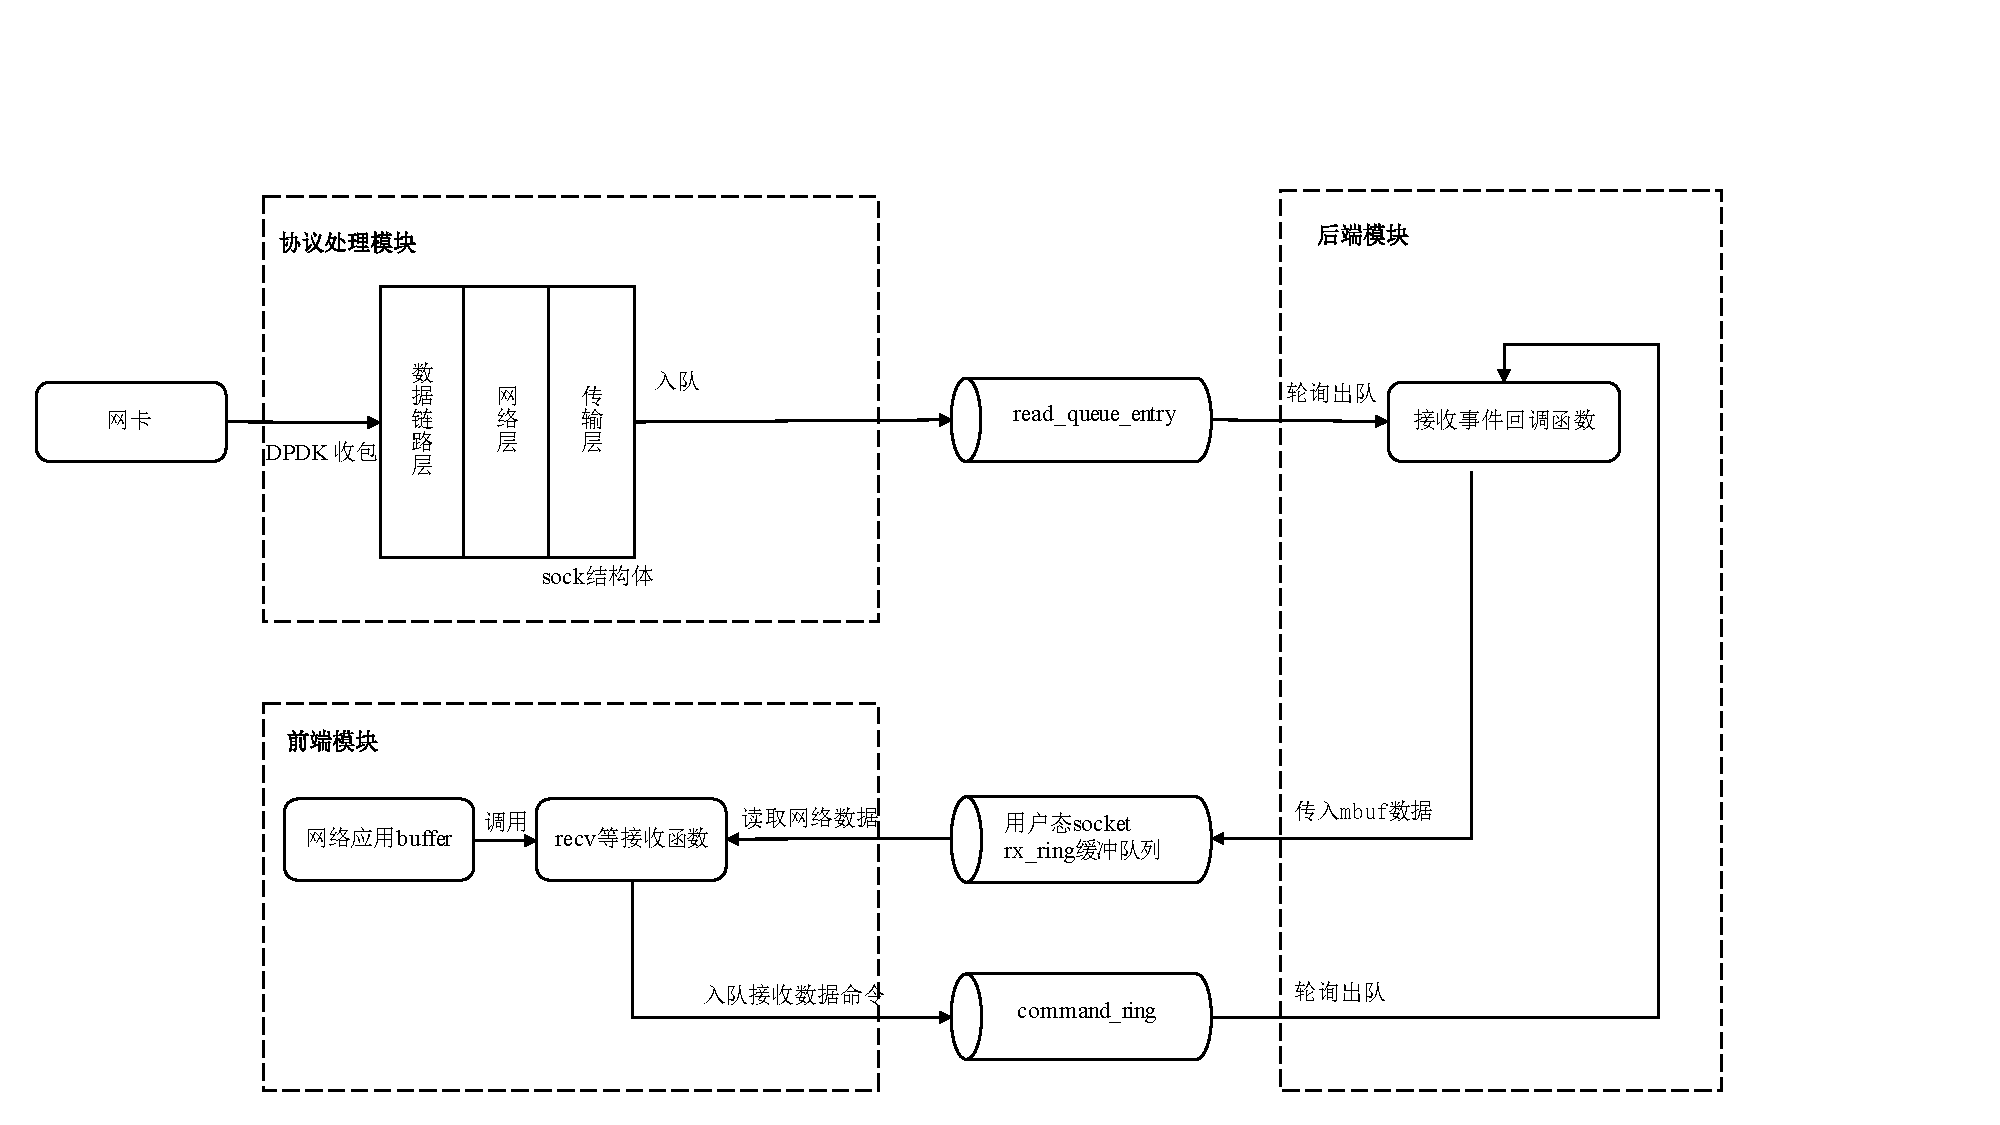
\includegraphics[width=\textwidth]{recv}
  \caption{用户态协议栈数据接收流程}
  \label{fig:recv}
\end{figure}
\vspace{-10pt}

\vspace{-10pt}
\begin{figure}[H] % use float package if you want it here
  \centering
  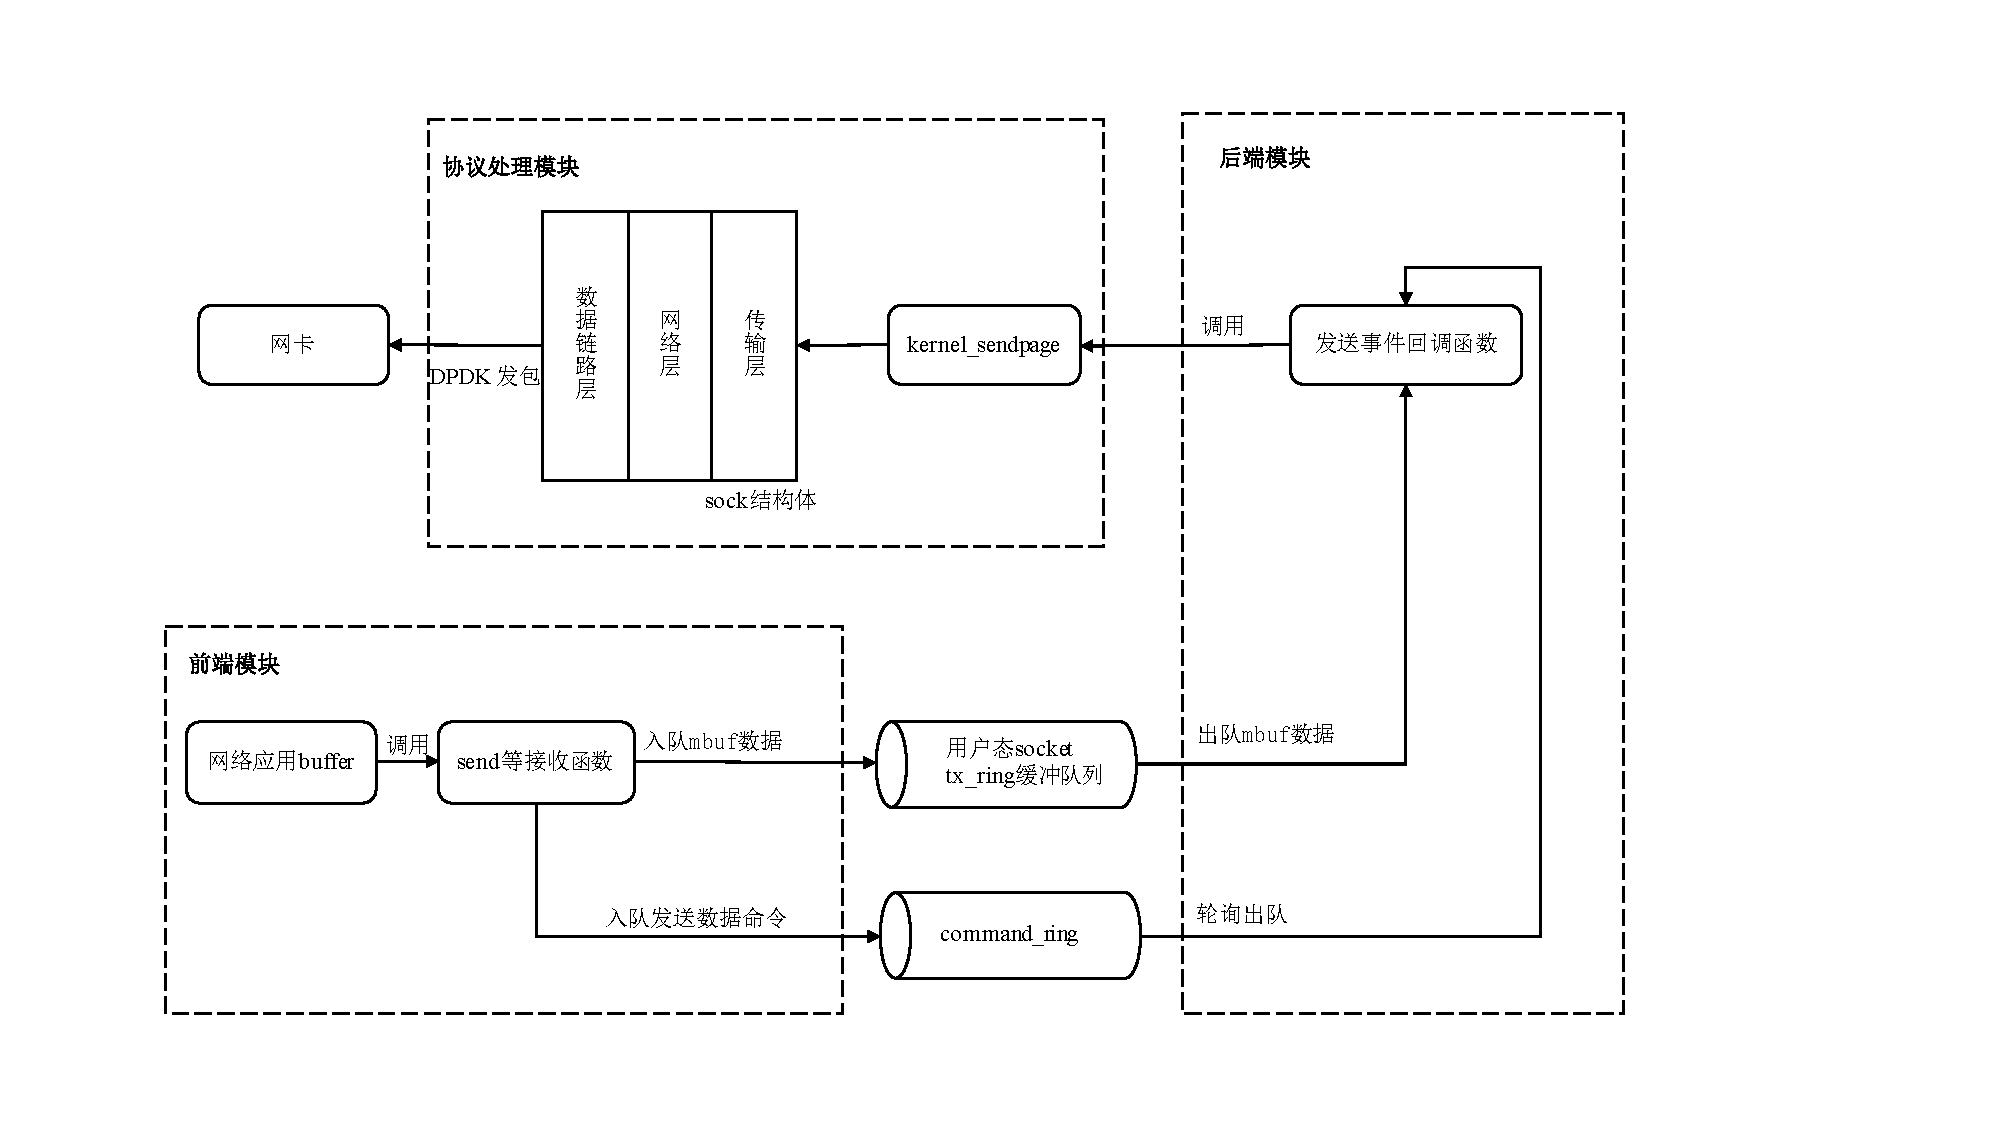
\includegraphics[width=\textwidth]{send}
  \caption{用户态协议栈数据发送流程}
  \label{fig:send}
\end{figure}
\vspace{-10pt}